\title{Scale-Sensitive Load Balancing for Numerically Multi-scale Simulations}
\author{W.R. Tobin, D. Fovargue, V.W.L. Chan, M.S. Shephard}
\date{\today}
\documentclass[11pt]{siamltex1213}
\bibliographystyle{siam}

\usepackage{graphicx}
\usepackage{mathtools}
\DeclarePairedDelimiter\ceil{\lceil}{\rceil}
\DeclarePairedDelimiter\floor{\lfloor}{\rfloor}

\begin{document}
\maketitle

\begin{abstract}
\end{abstract}

\section{Note}\label{note}
While this article predominantly discusses multi-scale simulations - wherein two or more separate physical scales are involved in the simulation - the discussion is equally applicable to multi-model simulations - wherein two or more numerical or physical models operating on the same domain (possibly with different discretizations) are involved in the simulation - as well as to multi-scale-multi-model simulations.

\section{Introduction}\label{introduction}
\label{single_scale_simulations}
Most physical models and implementations using numerical methods operate at a single scale characteristic to the problem. The scale at which the preponderance of attributes governing the underlying physics being modeled are measured and the resolution of the solution is considered commensurate with the desired accuracy of the simulation.

\label{multi_scale_simulations}
Introduction of influence from scales orders of magnitude removed from the primary scale can take place in several different ways. This influence can be incorporated during the mathematical development of the physical model itself. In this case the multi-scale features are incorporated into the numerical implementation automatically, as a result of their presence in the mathematical model. 

Multi-scale influences can also be incorporated in a more strictly numerical sense, combining physical models operating at different scales referencing and effecting shared physical fields and values \cite{shenoy97} \cite{weinan2003heterogenous}. Numerically multi-scale simulations associate many numerical implementations of single-scale physical models and cause them to interact in a meaningful way by passing key physical terms between scales, typically this will involve up-/down-scaling equations to take into account the difference in scale, refered to as compression and reconstruction operators in \cite{weinan2003heterogenous} for up-scaling and down-scaling, respectively. 

In order for a numerically multi-scale approach to be efficacious the domain at the scale of interest (for brevity the engineering scale) must be sufficiently large that conducting the entire simulation with terms and granularity orders of magnitude smaller would make the simulation computationally intractable. Thus some computationally reasonable subset of the engineering scale is assigned tertiary scales to simulate. The precise choice of location of the tertiary simulations is largely dependent on the specific numerical algorithms used to implement the engineering scale simulation. 

Typically the tertiary scale domain subset is related to locations in the engineering domain where the impact of the tertiary scales has the most impact on the engineering scale simulation. 

\label{multiscale_paradigms}
Among numerically multi-scale simulations, there are two primary paradigms: concurrent and sequential multi-scale. 

The sequential multi-scale paradigm involves the precomputation of parameters using a microscale simulation. These parameters are then used in a constitutive model for the macro-scale simulation \cite{garcia2008sequential}.

In the concurrent multi-scale paradigm, both scales are computed simultaneously and the required inter-scale coupling values are provided just-in-time \cite{zeng2010concurrent}.

\subsection{Load Balancing}\label{load_balancing}

\label{parallel_scaling}
As problem sizes grow - whether in terms of the underlying physical model used to simulate the problem or the granularity of the domain discretization or problem domain itself - single-scale simulations must be conducted on massively parallel machines in order to achieve meaningfully responsive results. This is accomplished by distributing problem data across the execution space of the machine, and keeping communication/blocking points to a minimum. 

\label{load_balancing_explained}
In order to maximize the computational gain granted by parallelization, load balancing must be used. The general load balancing problem depends on the implementation of the model used in a simulation; in terms of the data/tasks to be balanced as well as the necessary coordination between processes in order to advance the simulation. Further, the characteristics of the machine must be taken into account, both with respect to the hetero/homogeneity of the computational resources of the machine and the communications facilities employed. Finally combining the other dependencies, the load being balanced must have some metric denoting the computational demand associated with the discrete units capable of being distributed across the machine, as well as (possibly) the communication cost associated with that distribution. For a more in-depth discussion of load balancing theory, see \cite{} \cite{} \cite{}.

\label{single_scale_load_balancing}
Dynamic load balancing is a difficult problem, though many widely-used numerical methods and/or specific implementations of methods have developed relatively mature load balancing algorithms or heuristics \cite{Devine05}. In particular the finite element method - used in the primary scale of the Biotissue problem - has a mature set of load-balancing methods based on graph methods \cite{} \cite{} \cite{} \cite{}  used to distribute entities of the discretized domain and associated tensor field values across the execution space. The computational demand on each node can be estimated as a function of the number of individual elements that must be processed by each node, but due to dynamic mesh refinement processes used to minimize error estimators across the numerical problem domain, the global number of elements associated with the discretization may vary wildly over the course of a multi-load step simulation \cite{}. 

\label{scale_sensitive_load_balancing}
Using numerical methods for which load balancing schemes have been developed in a multi-scale simulation introduces a new set of complex constraints to the problem, due primarily to inter-scale dependencies. While it may be the case that such dependencies can be ignored, as in the case where all associate scales - those scales in the simulation which share a one- or two-way communication relationship with a given scale - must be fully reconstructed following a load-balancing operation. This reduces to the single-scale load balancing problem with an additional phase to reinitialize associate scales. When it is not possible to destroy or reinitialize associate scales, inter-scale dependencies must be maintained in order to continue computation. This operation is refered to as scale-sensitive load balancing, as only a single scale in a simulation is being considered while maintaining the validity of the global simulation.

\label{scale_balancing}
Beyond this introduction of new constraints to load balancing operations at each scale in a multi-scale system, the multi-scale system as a whole may greatly benefit from the use of scale-balancing. Scale-balancing is the balancing of scale-tasks against each other to minimize rendezvous time and maximize time spent in useful computation. Scale-balancing is a difficult prospect as it involves managing many dynamically-changing scales which themselves are being load-balanced using scale-sensitive load-balancing techniques, and represents a significant and promising area of future work.

\subsection{Adaptive Multi-scale Simulation Infrastructure}\label{amsi}
The Adaptive Multi-scale Simulation Infrastructure (amsi) is a set of libraries and tools developed at the Scientific Computation Research Center (SCOREC) at Rensselaer Polytechnic Institute. Amsi is designed to support the implementation and execution of dynamic numerically multi-scale simulations on massively-parallel HPC machines. Currently amsi provides interfaces for describing and managing the execution of individual scales in a multi-scale simulation, for defining and managing the scale-coupling communication required by such simulations, and for planning and enacting scale-sensitive load balancing operations on individual scales in a multi-scale system. 

Amsi operates by maintaining a set of minimal simulation metadata in order to model various quantities of interest during simulation execution. A decentralized approach toward control is taken; dynamic control decisions are made and implemented at runtime during collective operations. In order to avoid the introduction of unnecessary parallel barriers into the code, amsi control decisions are only made during operations which are already collective over the set of processes effected by a given control decision.

\label{amsi_scales}
During simulation initialization simulation scales are declared and then defined by associated them with process sets, and declaring their scale-linking relations. 

Process sets are simply mathematical sets of process ranks implemented so as to take advantage of any mathematical conveniences to minimize explicit storage whenever possible. At present process sets must be non-overlapping to take advantage of the simulation control mechanisms currently implemented in the amsi libraries, but for the simulation metadata modeling, scale-coupling communication, and multi-scale load balancing operations, the process sets associated with related scales may overlap, but simulation control must be explicitly handled by the simulation. 

Scales are declared to be related if some quantities of interest (such as tensor field values) are transmitted between them for scale-coupling. This coupling relationship is not assumed to be symmetric, thus if scale A is related to scale B, scale B is not implicitly related to scale A, though this may be seperately declared. 

\label{amsi_communication}
Scale coupling communication is handled by the amsi system using data distributions and communication patterns. A data distribution is a meta representation of individual units of scale-coupling data distributed across a single scale-task. The implementation of the coupling data is arbitrary (so long as it can be serialized for communication). A data distribution represents the smallest unit of data important to the scale-coupling communication, which is necessarily distinct for various multi-scale use cases.

\label{amsi_load_balancing}
If a local installation of the Zoltan \cite{ZoltanOverviewArticle2002} \cite{ZoltanIsorropiaOverview2012} load balancing library is available, the load balancing planning algorithms of Zoltan can be used underlying the scale-sensitive load balancing planning of amsi. A minimal set of load-balancing algorithms are provided with amsi. Since there is no general solution to the dynamic load balancing problem any set of provided load-balancing algorithms will prove insufficient for some use case. Thus amsi provides users with the ability to create and register their own load-balancing algorithms specific to the requirements of a given numerical implementation.

Due to the necessity of retaining inter-scale linkages through the load-balancing processes, the actual data migration undertaken to implement a specific load balancing plan is typically conducted internally by the amsi system which is provided with buffers of data being load-balanced by each process on the appropriate scale. However, in order to maintain usability in more general situations, it is also possible to simply inform the amsi system that the current load-balancing plan has already been accomplished by user-implemented data migration. This functionality combined with the ability to use user-designed load-balance planning algorithms allows amsi to work with entirely external load-balancing libraries and algorithms, allowing scale-sensitive load-balancing to be used even when a specific multi-scale use case falls outside the bounds of capabilities built into the system.

\label{amsi_scale_balancing}

\section{Load Balancing Approach}\label{methods}

\subsection{Scale-Sensitive Load Balancing}
\label{scale_sensitive_lb}
Scale-sensitive load balancing is a three-phase process: a planning phase, migration phase, and scale-syncing phase are required to complete a single load-balancing event.

\label{lb_planning}
The planning phase is a collective operation on the set of processes associated with the scale being load-balanced. During this phase weighting constraints and other information is provided to a planning algorithm which produces a plan for redistributing information such that the weighting metric is balanced. For this phase amsi typically utilizes planning algorithms provided by the Zoltan library, though as noted above any planning algorithm may be registered and used with the system. A simple example is provided is figure \ref{scale_sensitive_planning}, wherein each unit of load-balanced data has equal weight, a more concrete case will be discussed in section \ref{biotissue_load_balancing}.

\begin{figure}
  \begin{center}
    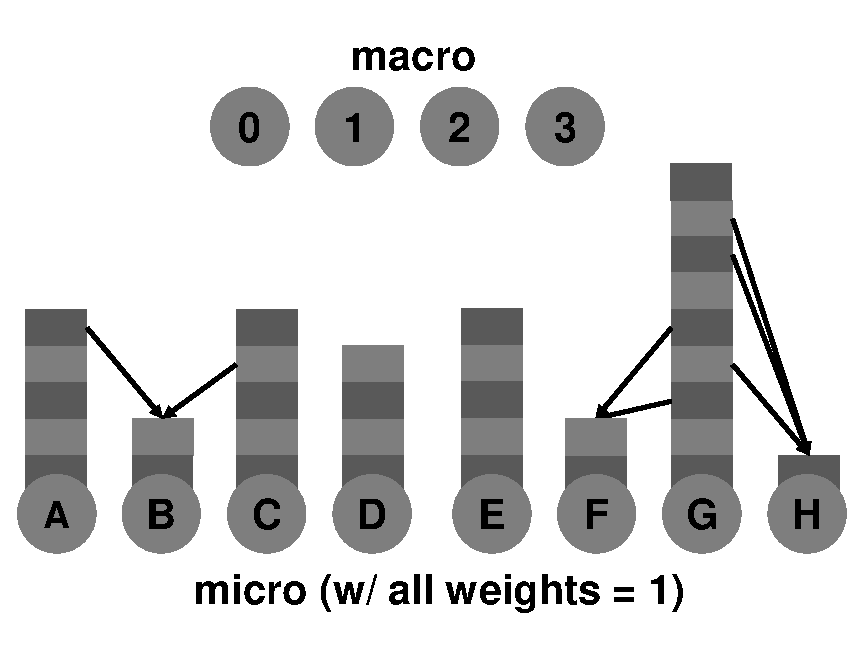
\includegraphics[height=2in]{scale_sensitive_lb_01.eps}
  \end{center}

  \caption{\small scale-sensitive load-balancing: planning}
  \label{scale_sensitive_planning}
\end{figure}

\label{lb_migration}
The migration phase is also collective on the set of processes associated with the scale being load-balanced. During this phase the plan from the previous step is put into action. Amsi provides support for automatic migration, if a user is able to provide a memory buffer of serialized load-balancing data in the same order as the weights were provided to the planning stage. The simple example continues in figure \ref{scale_sensitive_migration}. A user may also implement the migration function themselves and instead call the amsi migration interface with an empty buffer, which indicates the user has already completed the migration. This is necessary as there are minimal pieces of metadata (minimally two integers for each piece of migration data, which are typically appended during the amsi automatic migration and stripped off at the receiving end) which must be distributed by the amsi system for the third phase to complete.

\begin{figure}
  \begin{center}
    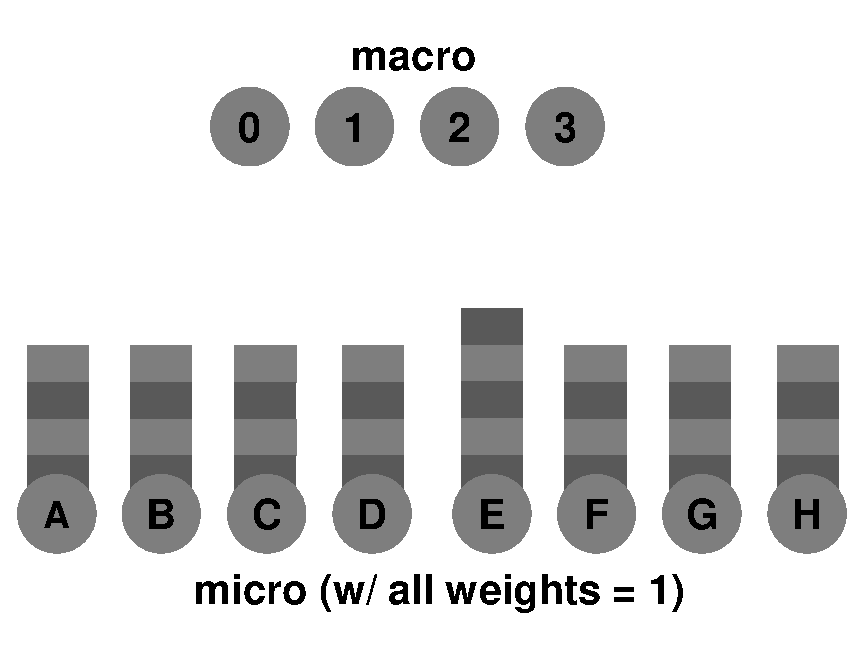
\includegraphics[height=2in]{scale_sensitive_lb_02.eps}
  \end{center}

  \caption{\small scale-sensitive load-balancing: migration}
  \label{scale_sensitive_migration}
\end{figure}

\label{lb_syncing}
The scale-syncing phase is collective over the set of process associated with the scale being load-balanced, and at least one associate scale. In this phase the appended metadata redistributed with the migration data is used to provide information to associate scales about the movement of the data at the scale being load-balanced. The simple example concludes in figure \ref{scale_sensitive_syncing}. Currently associate scales must interpret this data themselves - which consists of the scale-ranks of the origin and destination of the piece of data and the implicit ID assigned to the data due to its ordering in the migration buffer - but the implementation of domain relation metadata in the amsi system in the future should mitigate this requirement.

\begin{figure}
  \begin{center}
    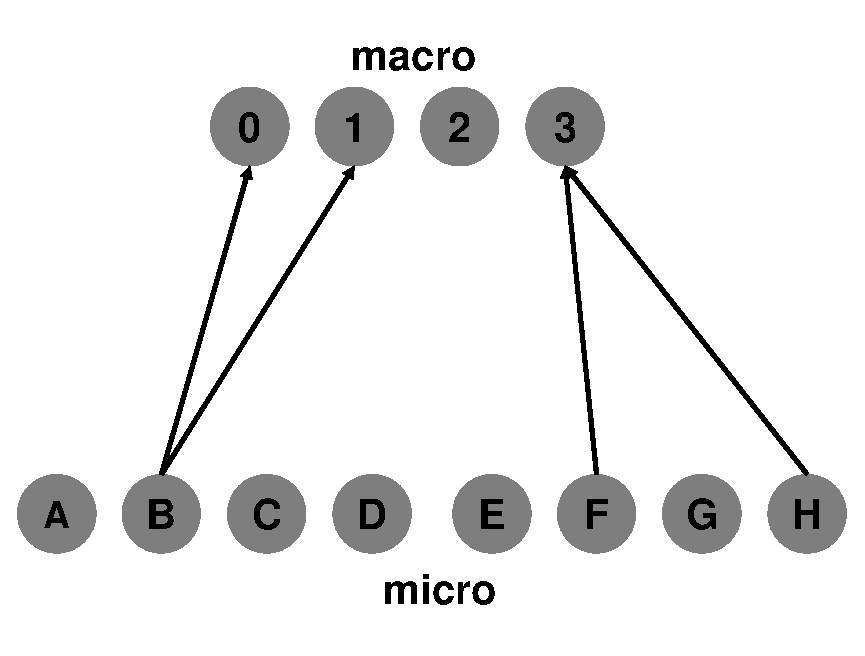
\includegraphics[height=2in]{scale_sensitive_lb_03.eps}
  \end{center}
  \caption{\small scale-sensitive load-balancing: scale-syncing}
  \label{scale_sensitive_syncing}
\end{figure}

\subsection{Example Problem: Biotissue}\label{biotissue}

The Biotissue code is a multi-scale simulation of soft organic tissues, consisting of an engineering-scale simulation using the finite element method, and a micro-scale quasistatics force-balance simulation. The Cauchy Momentum Balance Equation for a body in static equilibrium is used as the governing equation for the global simulation. Specific quantities needed to compute the elemental tangent stiffness matrices are instead supplied by the micro-scale force-balance simulations, which occur at each numerical integration point in the engineering-scale mesh, see figure \ref{biotissue_hierarchy}. 

\begin{figure}
  \begin{center}
    \includegraphics[height=2in]{biotissue_visual_hierarchy.eps}
  \end{center}

  \caption{\small biotissue multi-scale problem}
  \label{biotissue_hierarchy}
\end{figure}

The incremental displacements (the displacement deltas generated by the previous Newton iteration) on each engineering-scale finite element node are used to distort the a dimensionless representative volume element (RVE) resulting in each micro-scale node being displaced. Each RVE is a dimensionless unit cube containing a connected collagen fiber network, for the present results the fibers are implemented as truss elements and their distribution is generated using Delauney triangulation. The micro-scale boundary condition necessitates that the force exerted by each fiber network node located on the boundary of the RVE be zero. The micro-scale global Jacobian is formulated along with the force vector, wherein the boundary condition is enforced by setting specific rows of the force vector associated with boundary nodes to zero. 

Another Newton-Raphson iterative process occurs at micro-scale to converge to the set of displacements resulting in force equilibrium for all the fibers within the fiber network constituting the RVE. After a micro-scale simulation converges to a solution, the Jacobian and force vector are then evaluated again at the solution position, the force exerted along the boundary of the RVE is summed for each of the principal and shear components of a stress tensor, which is then dimensionalized and sent back to the engineering-scale for use in the elemental tangent stiffness matrix formulation. More detail into the derivation of this multi-scale system can be found in \cite{stylianopoulos2008thesis} \cite{agoram2001coupled} \cite{stylianopoulos2007multiscale} . Discussion of the dimensionalization of the dimensionless force terms produced by each fiber network can be found in \cite{stylianopoulos2007volume} \cite{chandran2007deterministic}.

%Typically in the displacement-based finite element method, a constitutive model depending on some set of material properties is derived from a set of governing physical partial differential equations. In the case of the Biotissue multi-scale code, the constitutive model governing the systemic response to the boundary conditions is supplemented by the micro-scale force-balance simulation. The Newton-Raphson method is used to iterate to the solution for a particular loading state, and at each Newton iteration the global tangent stiffness matrix is assembled from elemental systems generated from each element in the engineering-scale mesh. In typically FEM the elemental system is derived from the governing material model used for the specific type of material being simulated; for the Biotissue code the necessary values are instead provided as 

Thus the simulation as a whole is essentially doubly nonlinear, as during each engineering-scale Newton iteration every micro-scale RVE must undergo a full Newton-Raphson convergence process. 

\subsection{Biotissue Scale-Sensitive Load Balancing}\label{biotissue_load_balancing}

Scale-sensitive load balancing is conducted on the micro-scale RVE distribution at locations in the code where communication bottlenecks are already present. This prevents the introduction of new bottlenecks which could result in reduced performance. Macro-scale Newton-iterations are the most frequently occuring multi-scale communication bottleneck at which we chose to conduct the load balancing operation, and macro-scale incremental load steps the least-frequent. These represent the two extreme cases considered in our analysis on the efficacy of the scale-sensitive load-balancing scheme adopted for the biotissue simulation.

Each micro-scale RVE simulation involves the assembly and solve of a linear system of equations on the order of 10,000 unknowns for each micro-scale Newton iteration. While the total solve time is dependent on the number of nonlinear iterations and the hardware executing the code, this system is sufficiently small that parallelization of the RVE code itself is unwarranted, as the introduction of communication overhead into the RVE solution process would result in decreased performance, despite the modest gain to computation time. However, as each RVE represents an independent task to be accomplished by the simulation, they may be freely distributed across the processes assigned to the micro-scale computation. The only restriction to their (re)distribution for load balancing purposes is that the relation to a specific macro-scale numerical integration point must be maintained. 

As each RVE is a nonlinear simulation their is no a-prior estimate of the computational load each RVE represents, so the optimal initial distribution is simply treating the weight of each RVE as 1. Thus each micro-scale process is assigned either $\floor*{\frac{\text{num\_rves}}{\text{num\_micro\_procs}}}$ or $\ceil*{\frac{\text{num\_rves}}{\text{num\_micro\_procs}}}$. Once the first load-balancing event is reached, regardless of the granularity at which load-balancing is occuring for a given case, each RVE has recorded the total number of newton iterations it has conducted since the previous load-balancing event. This number is used as a heuristic weighting metric to determine the computational load of each individual RVE. The iteration count metric was chosen as each iteration takes a similar level of work to complete, up to the difference in the number of RVEs for each unique fiber network. Further, assuming linear incremental loading, regions in the engineering-scale mesh located near stress concentrators will result in 'more interesting' boundary conditions for the micro-scale problems related to numerical integration points in that region, which may result in the RVE requiring more Newton iterations to converge to an adequate solution, since the boundary conditions may lie farther from the initial state of the RVE in the regime of convergence for the nonlinear problem.

\section{Results}\label{results}

\begin{figure}
  \begin{center}
    \includegraphics[height=2in]{biotissue_visual_hierarchy.eps}
  \end{center}

  \caption{\small biotissue problem domain}
  \label{biotissue_domain}
\end{figure}

All discussed results were based on simulations of the problem domain seen in \ref{biotissue_domain}, a model of a standard tensile-test sample. More relevant domains to this problem based on data sampled from actual biological tissue samples are being prepared for use with the simulation, and results related to executing on these domains with appropriate boundary conditions will be discussed in forthcoming articles, as discussion of these subjects falls outside the pervue of this article.

Fixed psuedo-timestep incremental loading was used in the macro-scale finite element formulation for all load-balancing cases presented. The incremental loading used for a specific problem induces the boundary conditions on the various micro-scale RVEs in the domain each macro-scale Newton iteration. Thus, ultimately, the convergence behavior associated with each micro-scale RVE is wholly driven by the macro-scale incremental loading. 

\subsection{False Start}
The choice of weighting metric was encouraged by initial results for the statically distributed case (treating each RVE as though it had constant weight 1), as can be seen in \ref{init_results}. Each sub-chart in \ref{init_results} is associated with a single macro-scale incremental load step, and each bar represents the weight associated with a single micro-scale process during the execution of the macro-scale load step. 

\begin{figure}
  \begin{center}
    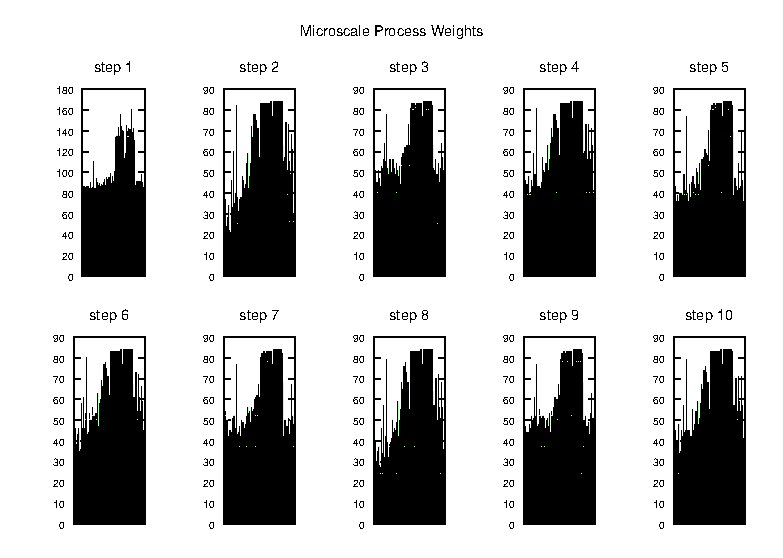
\includegraphics[height=2in]{init_results.eps}
  \end{center}

  \caption{\small flawed weight distribution - static}
  \label{init_results}
\end{figure}

The weight distribution observed retained a distinct pattern throughout the simulation. The existence of this pattern suggested that the motivation behind using the accumulated previous Newton-iteration count as the weighting metric could indeed be effective in achieving load balance. However, further examination of these initial results revealed a flaw in the micro-scale logic that sometimes prevented the micro-scale Newton-iterations from starting. This resulted in the initial fiber configuration - generated by the multi-scale coupling terms sent to the micro-scale RVE from the corresponding macro-scale element - being used as the final fiber configuration. While the simulation still converges in such a situation, the result is not characteristic of the expected response of the system. 

\begin{figure}
  \begin{center}
    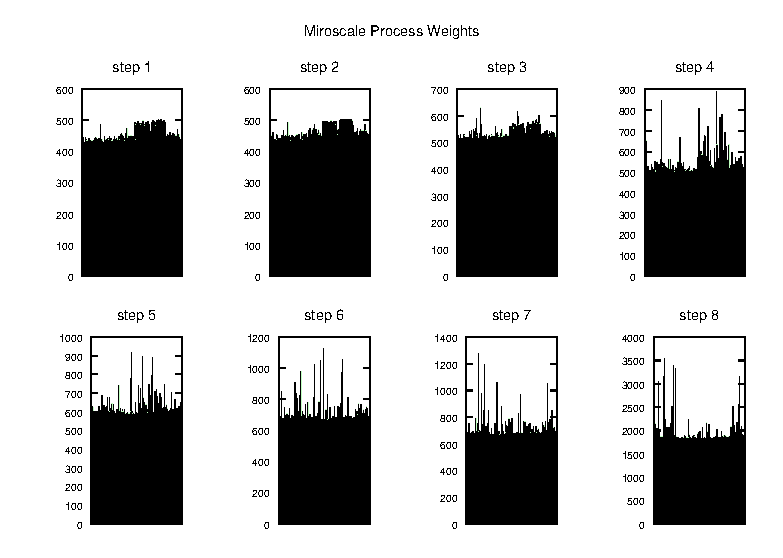
\includegraphics[height=2in]{fixed_results.eps}
  \end{center}

  \caption{\small corrected weight distribution - static}
  \label{fixed_results}
\end{figure}

\begin{figure}
  \begin{center}
    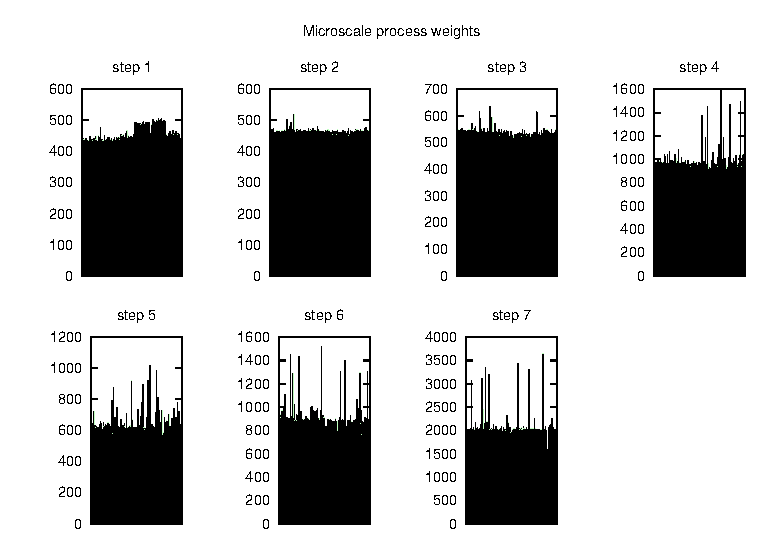
\includegraphics[height=2in]{fixed_results_lb.eps}
  \end{center}

  \caption{\small corrected weight distribution - dynamic}
  \label{fixed_results_lb}
\end{figure}


Upon repeating the simulation with the corrected micro-scale logic the corrected weight distribution and evolution throughout the simulation no longer exhibited this characteristic pattern as observed in the initial results \ref{fixed_results}. Thus the previous macro-scale load step's accumulated micro-scale Newton iterations do not represent an useful metric, even in a heuristic sense, of the convergence behavior of the associated RVE in the subsequent macro-scale load step. This can be seen in \ref{fixed_results_lb}, where clearly the load is not more balanced, in some cases the maximum deviation from the average is better then the corresponding case in the statically-balanced case, but it is also worse in many cases, and therefor ineffective in achieving performance gain under any metric.

The time-to-solution for the statically-loaded case - shown in \ref{fixed_results_timeline} - highlights the typical operation of each scale in the simulation. When any process associated with a scale is blocked, the scale is considered idle and shown in red, otherwise the scale is considered active and shown in green. The dynamically load balanced case is shown in \ref{fixed_results_lb_timeline}... [analysis of timelines]

\subsection{Per-Iteration Load Balancing}
While the discussed weighting metric might not be an accurate measure of the work in the upcoming macro-scale incremental load step, it may provide insight into the convergence properties of the RVE during the next macro-scale Newton-iteration during the same macro-scale incremental load step. Thus the load-balancing operation was altered to occur prior to every macro-scale Newton-iteration. Load-balancing occurs much more frequently and the global load being balanced is significantly smaller. Using this scheme we achieve the results seen in \ref{inter_newton_lb_results}.

\section{Future Work}\label{future_work}

Work on scale-balancing is ongoing for the Biotissue test problem. Using this work as a basis, a set of algorithms to provide support for more general scale-balancing operations will be developed and packaged into amsi.

Embedded fiber-matrix RVEs seperately parallelized and incorporated into multi-scale model, used at most error-sensitive locations \cite{lake2012mechanics} \cite{zhang2013cross} \cite{zhang2013coupled}.

\bibliography{works_cited}

\end{document}
